\documentclass[a4paper,10pt]{article}
\usepackage{listingsutf8}
\usepackage{color}
\usepackage{scalefnt}
\usepackage{cancel}
\usepackage{picinpar}
\usepackage{graphicx}
\usepackage{amssymb}
\usepackage{amsmath}
\usepackage[brazilian]{babel}
\usepackage[utf8]{inputenc}
\usepackage[T1]{fontenc}
\usepackage{setspace}
\usepackage{caption}
\usepackage[left=2cm,right=2cm,top=3.0cm,bottom=3cm]{geometry}
\usepackage{siunitx}
\usepackage[colorlinks=true,linkcolor=black,linktoc=all, urlcolor=black]{hyperref}
\usepackage{indentfirst}
\usepackage[nottoc]{tocbibind}
\usepackage[fixlanguage]{babelbib}
\usepackage{caption}
\usepackage{subcaption}
\usepackage{mdwlist}
\usepackage{fancyhdr}
\usepackage{helvet}
\renewcommand{\familydefault}{\sfdefault}

\selectbiblanguage{brazilian}
\renewcommand{\lstlistingname}{Código}
\lstset{
    inputencoding=utf8,
    extendedchars=true,
    numbers=left,
    numberstyle=\tiny,
    frame=lines,
    captionpos=b,
    literate=
        {á}{{\'a}}1 {é}{{\'e}}1 {í}{{\'i}}1 {ó}{{\'o}}1 {ú}{{\'u}}1 {ù}{{\`u}}1%
        {Á}{{\'A}}1 {É}{{\'E}}1 {Í}{{\'I}}1 {Ó}{{\'O}}1 {Ú}{{\'U}}1%
        {à}{{\`a}}1 {è}{{\'e}}1 {ì}{{\`i}}1 {ò}{{\`o}}1 {ò}{{\`o}}1%
        {À}{{\`A}}1 {È}{{\'E}}1 {Ì}{{\`I}}1 {Ò}{{\`O}}1 {Ò}{{\`O}}1%
        {ä}{{\"a}}1 {ë}{{\"e}}1 {ï}{{\"i}}1 {ö}{{\"o}}1 {ü}{{\"u}}1%
        {Ä}{{\"A}}1 {Ë}{{\"E}}1 {Ï}{{\"I}}1 {Ö}{{\"O}}1 {Ü}{{\"U}}1%
        {â}{{\^a}}1 {ê}{{\^e}}1 {î}{{\^i}}1 {ô}{{\^o}}1 {û}{{\^u}}1%
        {Â}{{\^A}}1 {Ê}{{\^E}}1 {Î}{{\^I}}1 {Ô}{{\^O}}1 {Û}{{\^U}}1%
        {ã}{{\~a}}1 {ẽ}{{\~e}}1 {ĩ}{{\~i}}1 {õ}{{\~o}}1 {ũ}{{\~u}}1%
        {Ã}{{\~A}}1 {Ẽ}{{\~E}}1 {Ĩ}{{\~I}}1 {Õ}{{\~O}}1 {Ũ}{{\~U}}1%
        {œ}{{\oe}}1 {Œ}{{\OE}}1 {æ}{{\ae}}1 {Æ}{{\AE}}1 {ß}{{\ss}}1%
        {ç}{{\c c}}1 {Ç}{{\c C}}1 {ø}{{\o}}1 {å}{{\r a}}1 {Å}{{\r A}}1%
        {€}{{\EUR}}1 {£}{{\pounds}}1,
}

\date{}
\title{
    Uma Ferramenta de Software para a Predição de Desempenho de Workflows Científicos\footnote{Este trabalho foi financiado por uma bolsa de iniciação científica CNPq/PIBIC (processo: 155544/2013-6).}
}

\author{
\textbf{\textit{Lucas Magno}}$^\dagger$,\textbf{ \textit{Kelly Rosa Braghetto}}$^\ddagger$\\
\\
\textit{Universidade de São Paulo} / $^\dagger$\textit{Instituto de Física,} $^\ddagger$\textit{Instituto de Matemática e Estatística}\\
\\
\href{mailto:lucas.magno@usp.br}{lucas.magno@usp.br} | \href{mailto:kellyrb@ime.usp.br}{kellyrb@ime.usp.br}
}


\fancyhf{} % sets both header and footer to nothing
\renewcommand{\headrulewidth}{0pt}
\cfoot{SIICUSP 2014 -- 22º Simpósio Internacional de Iniciação Científica e Tecnológica da USP }

\pagestyle{fancy}

\begin{document}
    \maketitle
    \section*{Resumo}
        Experimentos científicos frequentemente lidam com grandes quantidades de dados e processos com altos custos computacionais, exigindo a análise de seus desempenhos através de métodos que não envolvam suas execuções. Um destes métodos é a representação dos experimentos em modelos de \emph{workflow} por meio de linguagens formais, que permitem a extração de predições quantitativas de desempenho. Entretanto, o uso dessas linguagens requer familiaridade com formalismos complexos, restringindo-o às áreas da ciência com maior domínio em computação.

        Neste projeto, portanto, foi desenvolvida uma ferramenta em \emph{Python} capaz de, a partir da descrição de um \emph{workflow} em uma linguagem simples e intuitiva, gerar suas predições de desempenho através da álgebra de processos estocástica \emph{PEPA}, permitindo a otimização de experimentos científicos por usuários não-especialistas. 
    \section*{Abstract}

    \thispagestyle{fancy}

    \newpage
    \section*{Introdução}
        Inicialmente desenvolvidos para automatizar processos industriais e empresariais, os \emph{workflows} se popularizaram e passaram a ser usados na modelagem e automatização de experimentos científicos em diversas áreas da ciência. Um \emph{workflow científico} é a descrição completa ou parcial de um experimento científico em termo de suas atividades, controles de fluxo e dependência de dados \cite{phd:gadelha12}.

        Por ser comum em workflows científicos a manipulação de enormes quantidades de dados e a presença de processos que consomem muitos recursos computacionais, ferramentas que forneçam predições de desempenho desse tipo de sistema fazem-se necessárias. As predições auxiliam na escolha dos recursos computacionais apropriados para a execução e na identificação de possíveis problemas na modelagem dos workflows, possibilitando assim execuções mais eficientes.

        Há várias maneiras de se representar um \emph{workflow científico}, como, por exemplo, por meio de \emph{grafos direcionados}, \emph{UML \emph{(Unified Modeling Language)}}, \emph{redes de Petri} e \emph{álgebras de processos} \cite{phd:oga11}. Estes mecanismos de representação são usados para criar modelos que especificam a ordem de execução das atividades pertencentes aos \emph{workflows}. Linguagens formais como as redes de Petri e as álgebras de processos, vão além de uma simples representação, pois permitem também que se verifique propriedades qualitativas e quantitativas dos modelos de \emph{workflow} nelas representados. Em particular, extensões estocásticas dessas linguagens frequentemente são usadas para a criação de modelos preditivos do desempenho de sistemas computacionais.

        Apesar dos inúmeros benefícios que esses formalismos podem trazer à modelagem de workflows, o seu uso na prática impõe algumas dificuldades.  Ele exige que o usuário tenha familiaridade com linguagens e modelos estocásticos (de compreensão pouco intuitiva) e com seus programas de simulação ou análise numérica. No entanto, os \emph{workflows} científicos são criados e manipulados por cientistas das mais diversas áreas da ciência e que, geralmente, não são especialistas em computação.

    \section*{Objetivos}

    Este trabalho aborda o problema da predição de desempenho de workflows científicos, propondo uma ferramenta de software que automatiza a geração de predições baseadas em modelos estocásticos. O objetivo da ferramenta é esconder do usuário final a complexidade associada à criação e análise desse tipo de modelo.

     A ferramenta -- chamada de \texttt{wkf2pepa} -- gera automaticamente modelos estocásticos a partir de modelos de workflows descritos em uma linguagem bastante simples e de compreensão intuitiva, fácil de ser usada por cientistas de qualquer domínio. A ferramenta obtém a solução numérica dos modelos estocásticos e então extrai índices de desempenho relacionados aos modelos de workflows fornecidos como entrada.

    \section*{Materiais e Métodos}

        Os modelos de \emph{workflows} usados como entrada para a ferramenta \texttt{wkf2pepa} são descritos textualmente na forma de um grafo dirigido -- uma representação simples e que pode ser usada com facilidade por usuários não especialistas.
        Para a criação dos modelos estocásticos, optou-se pelo uso da linguagem \emph{PEPA -- Performance Evaluation Process Algebra}, uma álgebra de processos estocástica bem estabelecida e que conta com várias ferramentas de apoio.

         Neste trabalho, considera-se que \emph{workflows} sejam compostos por \emph{atividades}, que representam atividades reais de um experimento, e estruturas para descrever o fluxo de controle, como \emph{sequência}, \emph{paralelismo}, \emph{escolha} e \emph{sincronização}, definidas por meio dos operadores \emph{AND} (paralelismo/sincronização), \emph{XOR} (escolha exclusiva/junção) e \emph{OR} (escolha múltipla/junção).
        Para que possua um modelo correspondente em \emph{PEPA}, um modelo de \emph{workflow} precisa ser bem estruturado e não possuir ambiguidades semânticas. Por essa razão, neste trabalho são considerados apenas modelos de \emph{workflow} que apresentam somente um ponto de entrada e um ponto de saída, têm sua estrutura em forma de ``blocos'' e não apresentam ciclos, ou laços.

        A \texttt{wkf2pepa} foi implementada na linguagem \emph{Python}. Ela usa a bibllioteca \emph{pyPEPA}\cite{web:pypepa}, uma implementação recente de um solucionador para \emph{PEPA} em \emph{Python}, para calcular as probabilidades no regime estacion\'ario de cada um dos estados poss\'iveis do \emph{workflow} descrito no modelo em \emph{PEPA}. A partir dessas probabilidades, a \emph{pyPEPA} consegue fornecer o rendimento (\emph{throughput}) das atividades do \emph{workflow} e também a taxa de utilizaç\~ao de seus componentes.

        Além do modelo em \emph{PEPA} e sua solução, a \texttt{wkf2pepa} também gera uma representação gráfica do modelo de \emph{workflow}, que permite que o usuário possa verificá-lo mais facilmente.

        O funcionamento completo da ferramenta \texttt{wkf2pepa} pode ser descrito pelos seguintes passos:
        \begin{enumerate*}
            \item Recebe como entrada uma descrição textual (modelo) de um \emph{workflow} que segue uma sintaxe simples, criada com base na linguagem \emph{DOT} \cite{web:dot};
            \item Por meio de analisadores léxico e sintático gerados com a biblioteca \emph{PLY} (\emph{Python Lex-Yacc}) \cite{web:ply}, lê o modelo de workflow e gera uma representação em memória dele. Essa representação, baseada em grafos, é feita através de classes criadas na ferramenta para a manipulação de nós, arestas e \emph{workflows}.
            \item Gera uma descrição do \emph{workflow} de entrada em linguagem \emph{DOT} e sua representação gráfica (visualização) através da biblioteca \emph{Graphviz} \cite{web:graphviz}.
            \item Gera um modelo analítico (estocástico) do \emph{workflow} na linguagem \emph{PEPA}.
            \item Gera a solução numérica do modelo analítico e extrai os índices de desempenho com a  \emph{pyPEPA} .
        \end{enumerate*}


    \section*{Resultados}

    O código fonte da \texttt{wkf2pepa}, suas dependências, informações sobre o seu uso, exemplos de \emph{workflows} de entrada (e seus respectivos modelos em \emph{PEPA}) podem ser vistos na página do projeto \cite{web:script}.

    Ao processar um \emph{workflow}, a ferramenta cria arquivos de saída contendo a descrição do \emph{workflow} em \emph{DOT}, sua representação gráfica, sua descrição em \emph{PEPA} e os índices de desempenho dela extraídos. Um exemplo de descrição de workflow que pode ser usada como entrada para a ferramenta e parte dos resultados de saída gerados para ela são mostrados  na Figura~\ref{fig:exemplo}. Outros exemplos de workflows com estruturas mais complexas e seus respectivos resultados encontram-se na página do projeto \cite{web:script}.

\begin{figure}[h]
        \centering

        \begin{subfigure}[b]{0.6\textwidth}
                \footnotesize
                \lstinputlisting[tabsize=1]{example}
                \normalsize
                (a) Descrição do workflow de entrada.\\

                    \scriptsize
                \lstinputlisting[tabsize=1]{example.pepa}
                \normalsize
                (b) Modelo em PEPA gerado.\\

        \end{subfigure}%
        ~~%
        \begin{subfigure}[b]{0.4\textwidth}
                \centering
                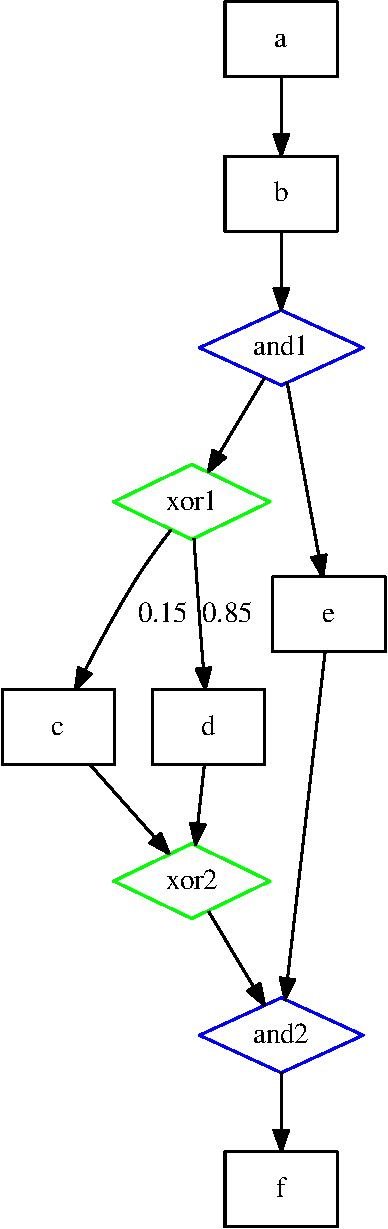
\includegraphics[scale=0.55]{example-crop.pdf}

                (c) Visualização criada a \\ partir da saída em DOT
                \label{fig:tiger}
        \end{subfigure}
        \caption{Exemplo de uma execução da \texttt{wkf2pepa}.}
        \label{fig:exemplo}
\end{figure}\\

    \newpage
    \section*{Conclusões}

    Este trabalho apresenta a ferramenta de software \texttt{wkf2pepa}, que converte de forma autom\'atica modelos de \emph{workflow} em modelos estocásticos e, a partir destes \'ultimos, extrai predições do desempenho dos \emph{workflows}. A predição do desempenho de workflows é importante porque auxilia a identificação de problemas em sua modelagem e o provisionamento dos recursos necessários para a execução eficiente desses sistemas.

    Os modelos de \emph{workflow} usados como entrada para a \texttt{wkf2pepa} são definidos por meio de uma notaç\~ao textual simples e intuitiva, que permite descrever as estruturas de fluxos de atividades mais comumente encontradas nos experimentos cient\'ificos. Assim, a \texttt{wkf2pepa} possibilita que usuários obtenham predições sobre o desempenho de workflows de forma prática, sem a necessidade de conhecer detalhes sobre modelagem estocástica e análise numérica.

    A \texttt{wkf2pepa} gera modelos estocásticos na álgebra de processos \emph{PEPA}. A ferramenta usa a biblioteca \emph{pyPEPA} para obter a solução numérica dos modelos estocásticos e índices de desempenho tais como a taxa de utilização dos componentes do modelo e o rendimento de cada atividade e do workflow como um todo.

    Como trabalhos futuros, pretende-se estender a \texttt{wkf2pepa} para que ela lide com modelos de workflows que incluam uma descrição dos recursos disponíveis para a execução. Com isso, os modelos estocásticos gerados e os índices de desempenho extraídos a partir deles fornecerão uma boa aproximação do desempenho real esperado para os workflows.


    \bibliographystyle{bababbr3}
    \bibliography{references}

\end{document}
